\section*{How does it work}

If you want to track an object, spherical markers can be added and Qualisys will be able to track it. These spherical markers can vary in size from 6.5mm to 19mm. In this project Qualisys will be used to track a quadcopter, registering the position and rotation. \\
\begin{figure}[h]
          \centering
            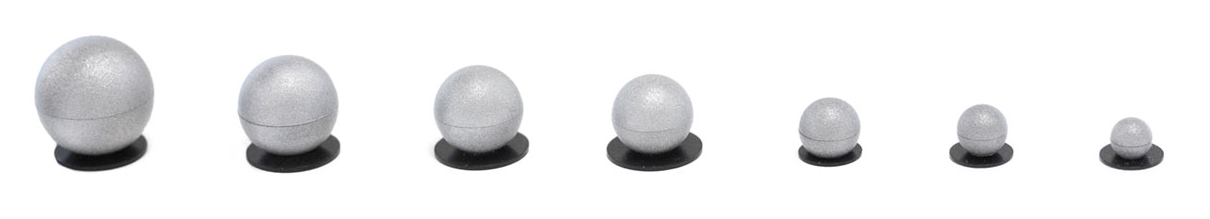
\includegraphics[scale = 0.35]{VAPIQ-PICTURES/sphere.png}
                \caption{Spherical markers to QTM}
                \label{sphere}
            \label{dir}
\end{figure}
\\
The input Qualisys needs is the spherical markers and it needs three markers in the same z-plane. The markers can give information about where it is and what direction the object is facing. Another marker is needed to be able to detect what is up and what is down. \\
\\
This information is sent on Wi-Fi to an external computer and can be displayed in the Qualisys Tracking Manager. The QTM is a GUI which displays the output from the cameras. The output given by Qualisys is the position of the quadcopter in x, y and z coordinates. The rotations are given by Euler angles ($ \phi,$ $ \theta $ and $ \psi $).\\
This information is displayed in the GUI giving a visualization of the position of the quadcopter. The GUI shows one coordinate system related to the room, and another coordinate system related to the body of the object.
\begin{figure}[ht]
          \centering
            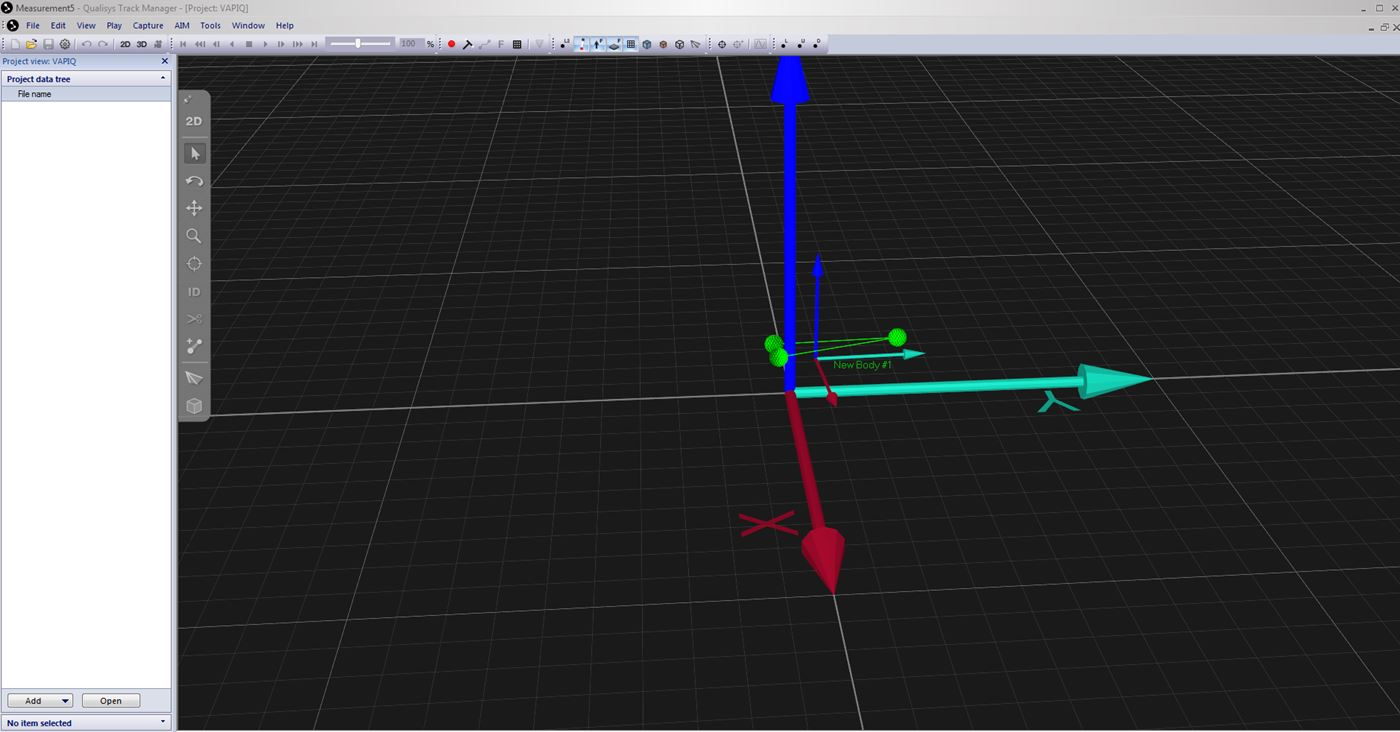
\includegraphics[scale = 0.25]{VAPIQ-PICTURES/qtm}
                \caption{Qualisys Tracking Manager 3D}
                \label{qtm3d}
            \label{dir}
\end{figure}
\newpage
However, to get the coordinate system of a quadcopter you need to configure the body reference. 
This is done by removing potential noise and confirming which marks are placed on the body. \\ 
\\
The AIM model (automatic identification of markers) can be added to any object that is tracked. It shows the connection between the different marks and can be animated in 3D.
The GUI helps with visualization and can ease testing. One can detect the route of a quadcopter in real-time or save the route to replay it for a more detailed study. 
\begin{figure}[h]
          \centering
            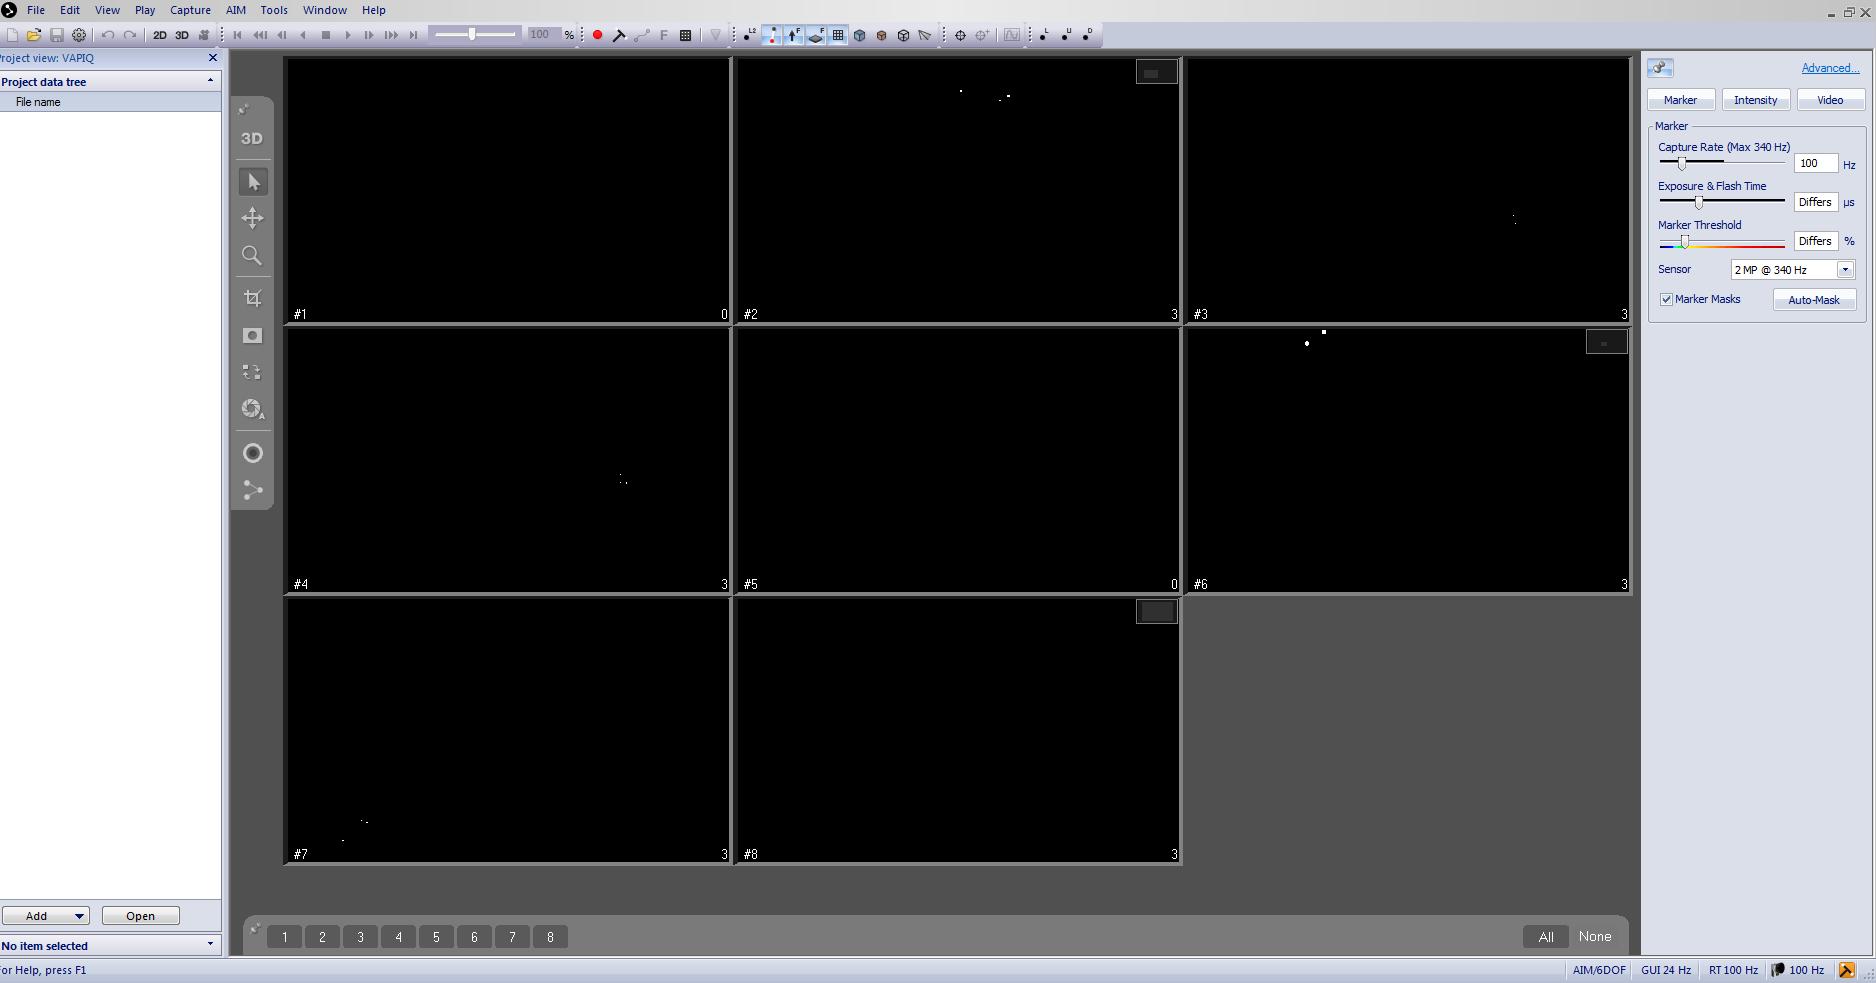
\includegraphics[scale = 0.25]{VAPIQ-PICTURES/qtm2d.png}
                \caption{Qualisys Tracking Manager 2D}
                \label{qtm2d}
            \label{dir}
\end{figure}
\\\\
\begin{figure}[h]
     \begin{minipage}[t]{0.45\textwidth}
    \textbf{Key features:}
        \begin{itemize}
            \item Optical real-time tracking
            \item Recordable
            \item Tracking in 2D, 3D and 6DOF
            \item Update frequency up to 340Hz
        \end{itemize}
     \end{minipage}
        \hfill
    \begin{minipage}[t]{0.45\textwidth}
        \textbf{System details:}
        \begin{itemize}
            \item Runs with Windows
            \item Wireless LAN option
            \item Compatible with matlab and avi 
            \item Single cable from cameras to computer
        \end{itemize}
    \end{minipage}
\end{figure}

